\section{1174054 - Aulyardha Anindita}

\subsection{Teori}
\begin{enumerate}
\item Jelaskan kenapa file teks harus dilakukan tokenizer. dilengkapi dengan ilustrasi atau gambar\\
Kata pada suatu teks disebut token. Proses vektorisasi dari bentuk kata kedalam token biasa disebut dengan tokenizer dan tokenizer tersebut akan merubah suatu teks tersebut menjadi simbol, kata, ataupun biner dan bentuk lainnya kedalam token. 
\hfill\break
	\begin{figure}[H]
		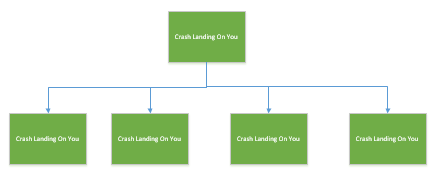
\includegraphics[width=4cm]{figures/1174054/7/1.png}
		\centering
		\caption{Tokenizer}
	\end{figure}

\item Jelaskan konsep dasar K Fold Cross Validation pada dataset komentar Youtube pada kode listing 7.1.dilengkapi dengan ilustrasi atau gambar.\\
StartifieldKFold berisi presentasi sampel dalam setiap kelas, dimana pada ilustrasi ini sampel tersebut dibagi menjadi 5 bagian dalam setiap classnya, lalu sampel tersebut dimasukkan kedalam class dari dataset youtube tersebut.
\hfill\break
	\begin{figure}[H]
		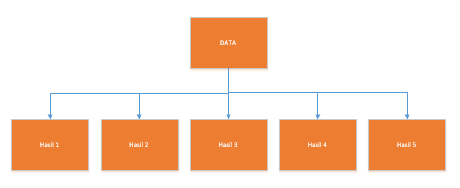
\includegraphics[width=4cm]{figures/1174054/7/2.png}
		\centering
		\caption{K-Fold Cross Validation}
	\end{figure}

\item Jelaskan apa maksudnya kode program for train, test in splits.dilengkapi dengan ilustrasi atau gambar\\
Maksud dari kode program for train, test in splits, yaitu menguji apakah setiap data pada dataset sudah displit dan tidak terjadi penumpukan, yang dimana setiap class tidak akan muncul dengan id yang sama. misalnya ketika kita akan mempunyai 4 tas dengan model yang berbeda, lalu kita membaginya menjadi dua anak, tentunya setiap anak tersebut akan menerima tas yang modelnya tidak sama.
\hfill\break
	\begin{figure}[H]
		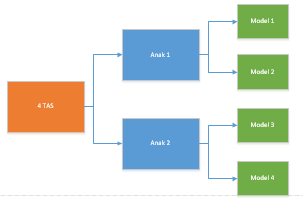
\includegraphics[width=4cm]{figures/1174054/7/3.png}
		\centering
		\caption{Maksud Kode dor train, test in splits}
	\end{figure}

\item Jelaskan apa maksudnya kode program train content = d[’CONTENT’].iloc[train idx] dan test content = d[’CONTENT’].iloc[test idx]. dilengkapi dengan ilustrasi atau gambar\\
Maksud dari kode program tersebut adalah mengambil data pada kolom atau index CONTENT yang merupakan bagian dari train idx dan test idx. Ilustrasinya, ketika data telah diubah menjadi train dan test maka kita dapat memilihnya untuk ditampilkan pada kolom yang diinginkan.
\hfill\break
	\begin{figure}[H]
		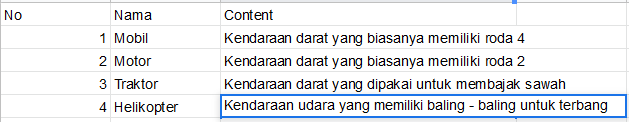
\includegraphics[width=4cm]{figures/1174054/7/4.png}
		\centering
		\caption{Maksud Kode train content}
	\end{figure}

\item Jelaskan apa maksud dari fungsi tokenizer = Tokenizer(num words=2000) dan tokenizer.fit on texts(train content), dilengkapi dengan ilustrasi atau gambar\\
Tokenizer(num words=2000) digunakan untuk membaca kalimat yang telah dibuat menjadi token sebanyak 2000 kata
tokenizer.fit on texts(train content) digunakan untuk membuat membaca data token teks yang telah dimasukkan kedalam fungsi yaitu fungsi train konten
\hfill\break
	\begin{figure}[H]
		
\includegraphics[width=4cm]{figures/1174054/7/5.png}
		\centering
		\caption{Maksud dari fungsi Tokenizer}
	\end{figure}

\item Jelaskan apa maksud dari fungsi d train inputs = tokenizer.texts to matrix(train content, mode='tfidf') dan d test inputs = tokenizer.texts to matrix(test content, mod='tfidf'), dilengkapi dengan ilustrasi kode atau gambar\\
Maksudnya yaitu untuk variabel d train inputs akan melakukan tokenizer dari bentuk teks kematrix dari data train content dengan mode matriksnya yaitu tfidf begitu juga dengan variabel d test inputs untuk data test. berikut gambar ilustrasinya:
\hfill\break
	\begin{figure}[H]
		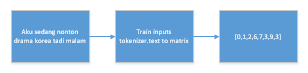
\includegraphics[width=4cm]{figures/1174054/7/6.png}
		\centering
		\caption{Maksud Kode train inputs}
	\end{figure}

\item Jelaskan apa maksud dari fungsi d train inputs = d train inputs/np.amax(np.absolute(d train dan d test inputs = d test inputs/np.amax(np.absolute(d test inputs)), dilengkapi dengan ilustrasi atau gambar.\\
Fungsi tersebut akan membagi matrix tfidf tadi dengan amax yaitu mengembalikan maksimum array atau maksimum sepanjang sumbu. Yang hasilnya akan dimasukkan kedalam variabel d train inputs untuk data train dan d test inputs untuk data test dengan nominal absolut atau tanpa ada bilangan negatif dan koma.
\hfill\break
	\begin{figure}[H]
		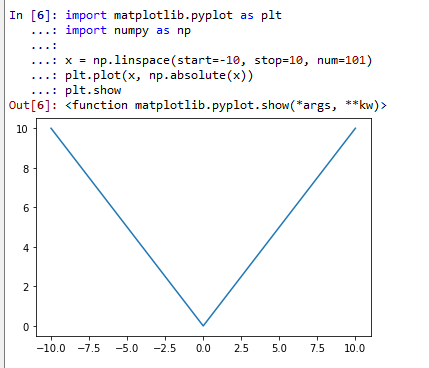
\includegraphics[width=4cm]{figures/1174054/7/7.png}
		\centering
		\caption{Maksud Kode train inputs}
	\end{figure}

\item Jelaskan apa maksud fungsi dari d train outputs = np utils.to categorical(d[’CLASS’].iloc[train dan d test outputs = np utils.to categorical(d[’CLASS’].iloc[test idx]) dalam kode program, dilengkapi dengan ilustrasi atau gambar.\\
Dalam variabe ld train output dan d test outputs akan dilakukan one hot encoding,dimana np utils akan mengubah vektor dengan bentuk integer ke matriks kelas biner untuk kolom CLASS dimana nantinya hanya akan ada dua pilihan yaitu 1 atau 0. 1 untuk spam 0 untuk non spam atau sebaliknya. Berikut gambar ilustrasinya :
\hfill\break
	\begin{figure}[H]
		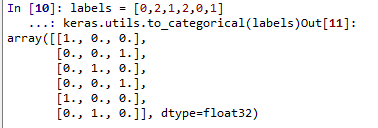
\includegraphics[width=4cm]{figures/1174054/7/8.png}
		\centering
		\caption{Maksud Kode train outputs}
	\end{figure}

\item Jelaskan apa maksud dari fungsi di listing 7.2. Gambarkan ilustrasi Neural Network nya dari model kode tersebut\\
Maksud dari listing 7.2 yaitu :
\begin{itemize}
\item melakukan pemodelan sequential
\item Layer pertama dense dari 512 neuron untuk inputan dengan inputan tadi yang sudah dijadikan matriks sebanyak 2000
\item Activationnya menggunakan fungsi relu yaitu jika ada inputan dengan nilai maksimum maka inputan itu yang akan terpilih.
\item Dropout ini untuk melakukan pembobotan, dimana pembobotan hanya dilakukan 50 persen saja agar tidak terjadi penumpukan data dari dense inputan tadi
\item Dense 2 mengkategorikan 2 neuron untuk output nya yaitu 1 dan 0.
\item Untuk dense diatas aktivasinya menggunakan fungsi Softmax. 
\end{itemize}
Untuk ilustrasinya bisa dilihat pada gambar berikut :
\hfill\break
	\begin{figure}[H]
		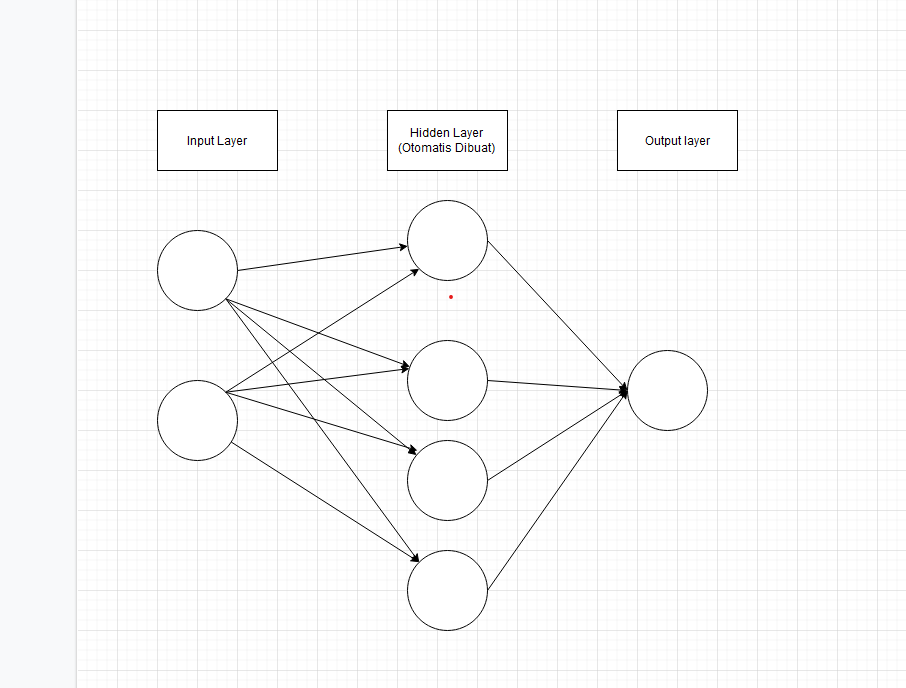
\includegraphics[width=4cm]{figures/1174054/7/9.png}
		\centering
		\caption{Ilustrasi Neural Network}
	\end{figure}

\item Jelaskan apa maksud dari fungsi di listing 7.3 dengan parameter tersebut.\\
Melakukan peng compile-an dari model Sequential tadi dengan Loss yan dengan merupakan fungsi optimisasi skor menggunakan categorical crossentropy,dan menggunakan algoritma adam sebagai optimizer. Adam yaitu algoritma pengoptimalan yang dapat digunakan sebagai ganti dari prosedur penurunan gradien stokastik klasik untuk memperbarui bobot jaringan yang berulang berdasarkan data training.Dengan metrik yaitu fungsi yang digunakan untuk menilai kinerja mode Anda disini menggunakan fungsi accuracy. 

\item Jelaskan apa itu Deep Learning\\
Deep learning merupakan salah satu algoritma yang seperti Neural Network yang menggunakan meta data sebagai inputan dan mengolahnya menggunakan layer layer yang tersembunyi.

\item Jelaskan apa itu Deep Neural Network, dan apa bedanya dengan Deep Learning\\
Deep Neural Network adalah jaringan syaraf tiruan (JST) dengan beberapa lapisan antara lapisan input dan output. DNN menemukan manipulasi matematis yang benar untuk mengubah input menjadi output, apakah itu hubungan linear
Deep Neural Network adalah jaringan syaraf tiruan (JST) dengan beberapa lapisan antara lapisan input dan output. DNN menemukan manipulasi matematis yang benar untuk mengubah input menjadi ouput, apakah itu hubungan linear atau hubungan non-linear. Merupakan jaringan syaraf dengan tingkat kompleksitas tertentu, jaringan syaraf dengan lebih dari dua lapisan. Deep Neural Network menggunakan pemodelan matematika yang canggih untuk memproses data dengan cara yang kompleks. DNN hanya terdiri dari dua lapisan yaitu input dan output, sedangkan dalam Deep learning kita dapat mendefinisikan layer sebanyak yang kita inginkan atau butuhkan.

\item Jelaskan dengan ilustrasi gambar buatan sendiri (langkah per langkah) bagaimana perhitungan algoritma kobvolasi dengan ukuran stride (NPM mod3+1) x (NPM mod3+1) yang terdapat pada max pooling\\
Karena hasil dari (NPM mod3+1) x (NPM mod3+1) = 2 x 2 = 4, berarti ada 4 metode max pooling, sebelum membuat ilustrasi perlu diketahui apa itu stride, stride adalag acuan atau parameter yang menentukan pergeseran pada filter fixcel, sebagai contoh nilai stride 1 yang berarti filter akan bergeser sebanyak satu fixcel secara vertikal dan horizontal. selanjutnya apa itu max pooling contoh pada suatu gambar ditentukan max pooling dari 3x3 dengan stride 1 yang berarti setiap pergeseran 1 pixcel akan diambil nilai terbesar dari pixcel 3 x 3 tersebut.
\begin{figure}[H]
		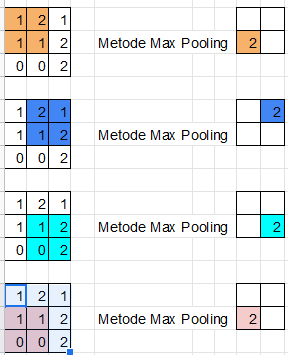
\includegraphics[width=4cm]{figures/1174054/7/10.png}
		\centering
		\caption{Illustrasi perhitungan stride 1 max pooling}
	\end{figure}

\end{enumerate}

\subsection{Praktek}
\begin{enumerate}
\item Nomor 1
\lstinputlisting[firstline=8, lastline=14]{src/1174054/7/1174054.py}
Dan hasilnya bisa dilihat pada gambar berikut :
\hfill\break
	\begin{figure}[H]
		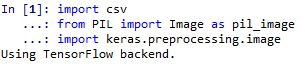
\includegraphics[width=4cm]{figures/1174054/7/11.png}
		\centering
		\caption{Hasil Nomor 1}
	\end{figure}

\item Nomor 2
\hfill\break
	\lstinputlisting[firstline=16, lastline=39]{src/1174054/7/1174054.py}
Untuk hasil plotnya bisa dilihat pada gambar berikut:
\hfill\break
	\begin{figure}[H]
		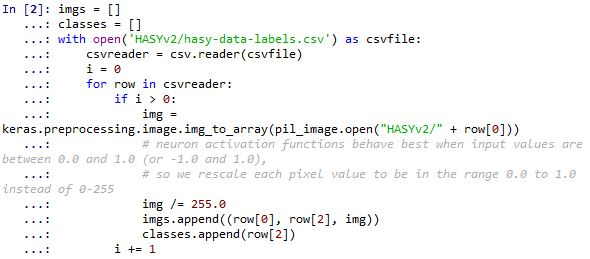
\includegraphics[width=4cm]{figures/1174054/7/12.JPG}
		\centering
		\caption{Hasil Nomor}
	\end{figure}
	
\item Nomor 3
\hfill\break
	\lstinputlisting[firstline=41, lastline=51]{src/1174054/7/1174054.py}
Hasilnya dapat dilihat pada gambar berikut:
\hfill\break
	\begin{figure}[H]
		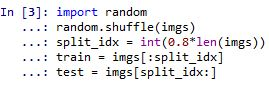
\includegraphics[width=4cm]{figures/1174054/7/13.JPG}
		\centering
		\caption{Hasil Nomor 3}
	\end{figure}
	
\item Nomor 4
\hfill\break
	\lstinputlisting[firstline=53, lastline=63]{src/1174054/7/1174054.py}
Untuk hasilnya bisa dilihat pada gambar berikut :
\hfill\break
	\begin{figure}[H]
		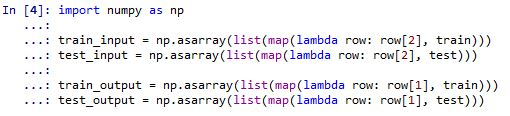
\includegraphics[width=4cm]{figures/1174054/7/14.JPG}
		\centering
		\caption{Hasil Nomor 4}
	\end{figure}	

\item Nomor 5
\hfill\break
	\lstinputlisting[firstline=65, lastline=69]{src/1174054/7/1174054.py}
Untuk hasilnya bisa dilihat pada gambar berikut :
\hfill\break
	\begin{figure}[H]
		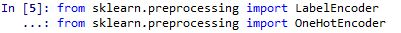
\includegraphics[width=4cm]{figures/1174054/7/15.JPG}
		\centering
		\caption{Hasil Nomor 5}
	\end{figure}
	
\item Nomor 6\\
\hfill\break
	\lstinputlisting[firstline=71, lastline=76]{src/1174054/7/1174054.py}
Hasilnya bisa dilihat pada gambar berikut :
\hfill\break
	\begin{figure}[H]
		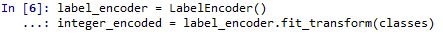
\includegraphics[width=4cm]{figures/1174054/7/16.JPG}
		\centering
		\caption{Hasil Nomor 6}
	\end{figure}
	
\item Nomor 7
\hfill\break
	\lstinputlisting[firstline=78, lastline=84]{src/1174054/7/1174054.py}
Hasilnya bisa dilihat pada gambar berikut :
\hfill\break
	\begin{figure}[H]
		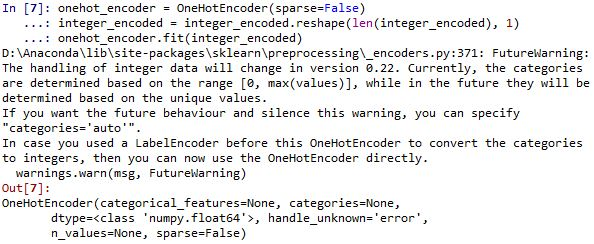
\includegraphics[width=4cm]{figures/1174054/7/17.JPG}
		\centering
		\caption{Hasil Nomor 7}
	\end{figure}
	
\item Nomor 8
\hfill\break
	\lstinputlisting[firstline=86, lastline=98]{src/1174054/7/1174054.py}
Untuk hasilnya bisa dilihat pada gambar berikut :
\hfill\break
	\begin{figure}[H]
		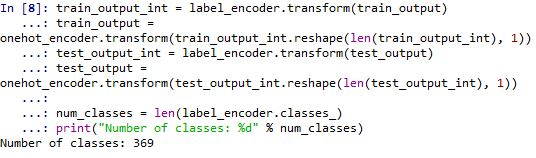
\includegraphics[width=4cm]{figures/1174054/7/18.JPG}
		\centering
		\caption{Hasil Nomor 8}
	\end{figure}
	
\item Nomor 9
\hfill\break
	\lstinputlisting[firstline=100, lastline=106]{src/1174054/7/1174054.py}
Hasilnya bisa dilihat pada gambar berikut :
\hfill\break
	\begin{figure}[H]
		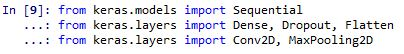
\includegraphics[width=4cm]{figures/1174054/7/19.JPG}
		\centering
		\caption{Hasil Nomor 9}
	\end{figure}
	
\item Nomor 10
\hfill\break
	\lstinputlisting[firstline=108, lastline=132]{src/1174054/7/1174054.py}
Hasilnya bisa dilihat pada gambar berikut :
\hfill\break
	\begin{figure}[H]
		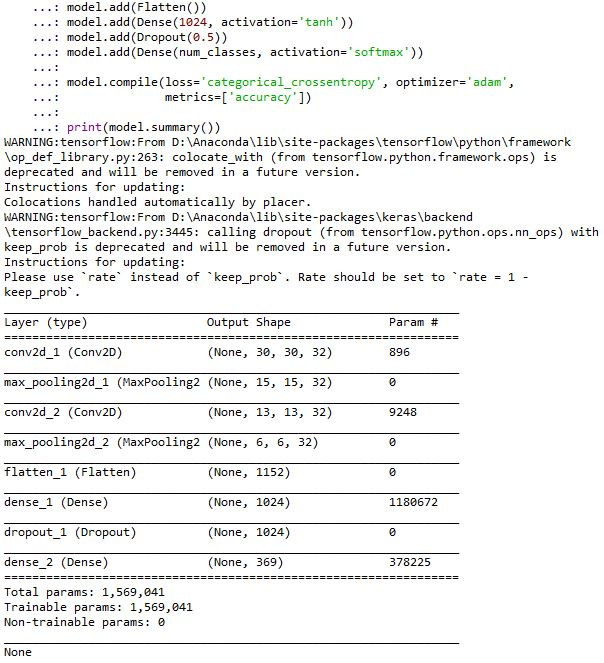
\includegraphics[width=4cm]{figures/1174054/7/20.JPG}
		\centering
		\caption{Hasil Nomor 10}
	\end{figure}
	
\item Nomor 11
\hfill\break
	\lstinputlisting[firstline=134, lastline=138]{src/1174054/7/1174054.py}
Hasilnya bisa dilihat pada gambar berikut :
\hfill\break
	\begin{figure}[H]
		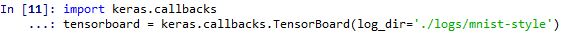
\includegraphics[width=4cm]{figures/1174054/7/21.JPG}
		\centering
		\caption{Hasil Nomor 11}
	\end{figure}
	
\item Nomor 12
\hfill\break
	\lstinputlisting[firstline=140, lastline=152]{src/1174054/7/1174054.py}
Hasilnya bisa dilihat pada gambar berikut :
\hfill\break
	\begin{figure}[H]
		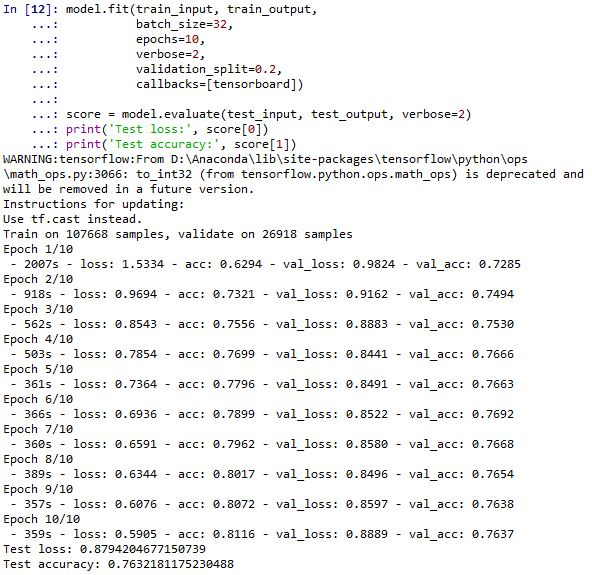
\includegraphics[width=4cm]{figures/1174054/7/22.JPG}
		\centering
		\caption{Hasil Nomor 12}
	\end{figure}
	
\item Nomor 13
\hfill\break
	\lstinputlisting[firstline=154, lastline=209]{src/1174054/7/1174054.py}
Hasilnya bisa dilihat pada gambar berikut :
\hfill\break
	\begin{figure}[H]
		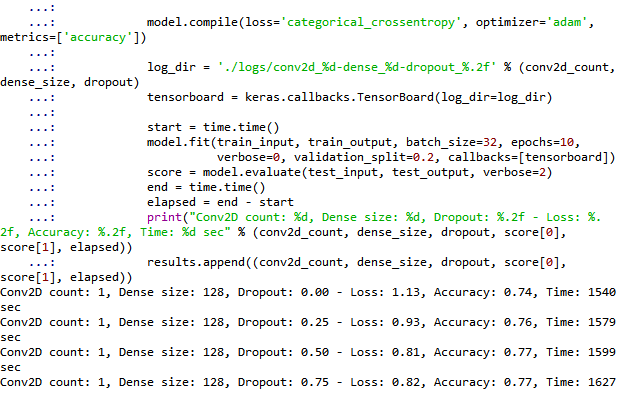
\includegraphics[width=4cm]{figures/1174054/7/23.PNG}
		\centering
		\caption{Hasil Nomor 13}
	\end{figure}
	
\item Nomor 14
\hfill\break
	\lstinputlisting[firstline=211, lastline=233]{src/1174054/7/1174054.py}
Hasilnya bisa dilihat pada gambar berikut :
\hfill\break
	\begin{figure}[H]
		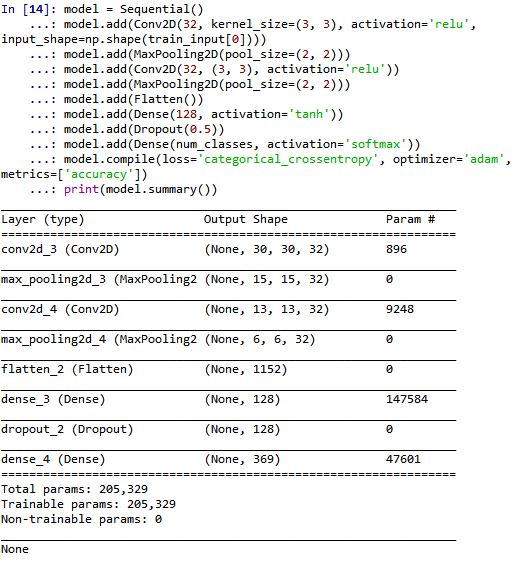
\includegraphics[width=4cm]{figures/1174054/7/24.JPG}
		\centering
		\caption{Hasil Nomor 14}
	\end{figure}
	
\item Nomor 15
\hfill\break
	\lstinputlisting[firstline=235, lastline=241]{src/1174054/7/1174054.py}
Hasilnya bisa dilihat pada gambar berikut :
\hfill\break
	\begin{figure}[H]
		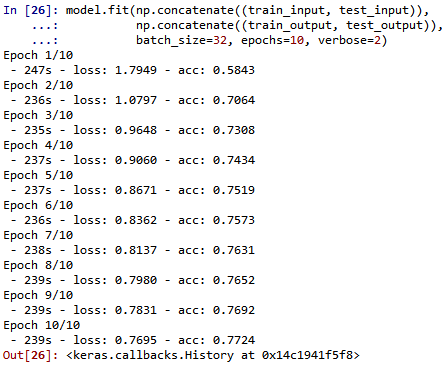
\includegraphics[width=4cm]{figures/1174054/7/25.PNG}
		\centering
		\caption{Hasil Nomor 15}
	\end{figure}

\item Nomor 16
\hfill\break
	\lstinputlisting[firstline=243, lastline=245]{src/1174054/7/1174054.py}
Hasilnya bisa dilihat pada gambar berikut :
\hfill\break
	\begin{figure}[H]
		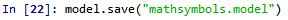
\includegraphics[width=4cm]{figures/1174054/7/26.JPG}
		\centering
		\caption{Hasil Nomor 16}
	\end{figure}
	
\item Nomor 17
\hfill\break
	\lstinputlisting[firstline=247, lastline=249]{src/1174054/7/1174054.py}
Hasilnya bisa dilihat pada gambar berikut :
\hfill\break
	\begin{figure}[H]
		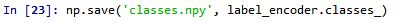
\includegraphics[width=4cm]{figures/1174054/7/27.JPG}
		\centering
		\caption{Hasil Nomor 17}
	\end{figure}
	
\item Nomor 18
\hfill\break
	\lstinputlisting[firstline=251, lastline=258]{src/1174054/7/1174054.py}
Hasilnya bisa dilihat pada gambar berikut :
\hfill\break
	\begin{figure}[H]
		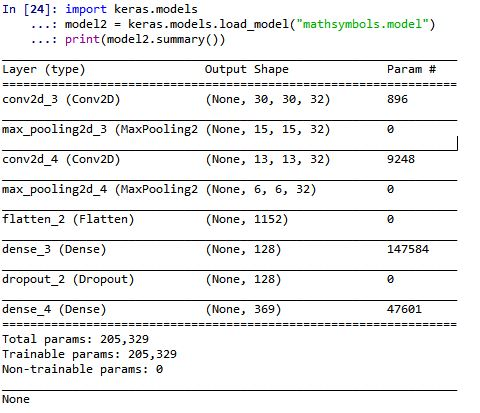
\includegraphics[width=4cm]{figures/1174054/7/28.JPG}
		\centering
		\caption{Hasil Nomor 18}
	\end{figure}
	
\item Nomor 19
\hfill\break
	\lstinputlisting[firstline=260, lastline=280]{src/1174054/7/1174054.py}
Hasilnya bisa dilihat pada gambar berikut :
\hfill\break
	\begin{figure}[H]
		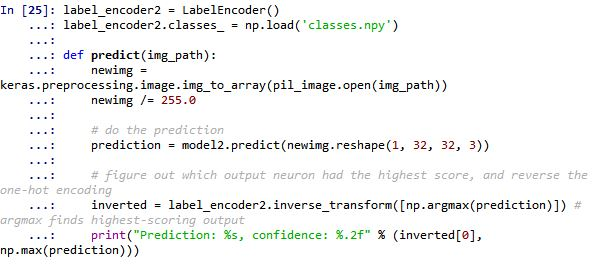
\includegraphics[width=4cm]{figures/1174054/7/29.JPG}
		\centering
		\caption{Hasil Nomor 19}
	\end{figure}
	
\item Nomor 20
\hfill\break
	\lstinputlisting[firstline=282, lastline=288]{src/1174054/7/1174054.py}
Hasilnya bisa dilihat pada gambar berikut :
\hfill\break
	\begin{figure}[H]
		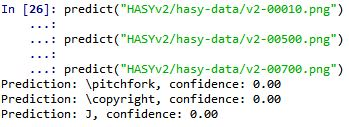
\includegraphics[width=4cm]{figures/1174054/7/30.JPG}
		\centering
		\caption{Hasil Nomor 20}
	\end{figure}	
	
\end{enumerate}

\subsection{Penanganan Error}
\begin{enumerate}
\item ScreenShoot Error
	\begin{figure}[H]
		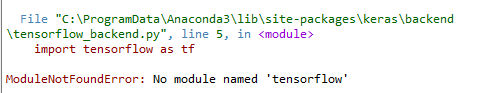
\includegraphics[width=4cm]{figures/1174054/7/error.png}
		\centering
		\caption{Module Not Found Error}
	\end{figure}

	\item Tuliskan Kode Error dan Jenis Error
	\begin{itemize}
		\item Module Not Found Error

	\end{itemize}
	\item Cara Penanganan Error
	\begin{itemize}
		\item Module Not Found Error
		\hfill\break
		Error terjadi karena belum menginstal package atau library tensorflow Untuk mengatasinya dengan mengisntal library tensorflow pada anaconda
	\end{itemize}
\end{enumerate}


\subsection{Bukti Tidak Plagiat}
\begin{figure}[H]
	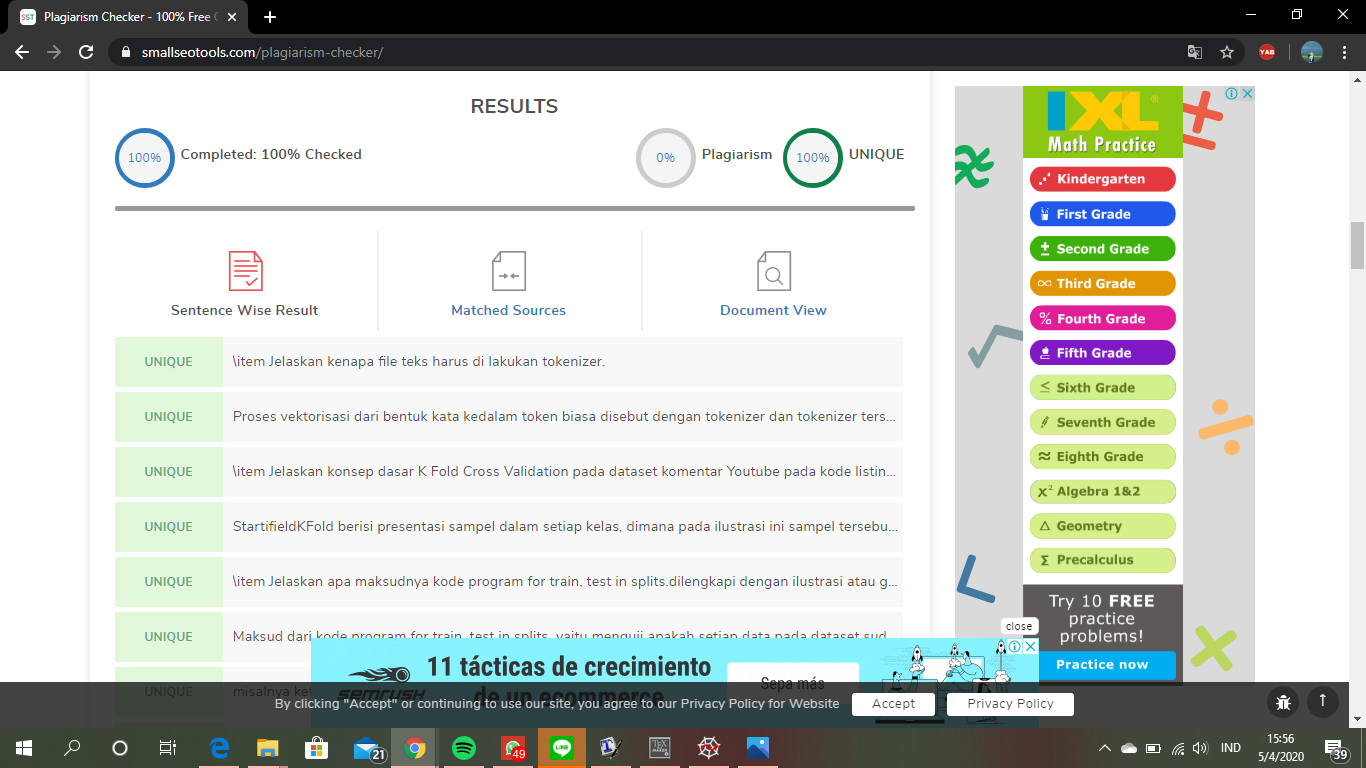
\includegraphics[width=4cm]{figures/1174054/7/plagiarisme.png}
	\centering
	\caption{Bukti Plagiasrisme}
\end{figure}

\subsection{Link Youtube}
https://youtu.be/5jv7jHYu7pg